\documentclass[11pt,reqno]{amsart}

\usepackage[margin=0.95in]{geometry}
\usepackage{amsmath,amssymb,amsthm}
\usepackage{booktabs}
\usepackage{tabularx}
\usepackage{array}
\usepackage{graphicx}
\usepackage{xcolor}
\usepackage{enumitem}
\usepackage{microtype}
\usepackage{placeins}
\PassOptionsToPackage{obeyspaces}{url}
\usepackage{xurl}
\usepackage{tikz}
\usepackage{pgfplots}
\pgfplotsset{compat=1.18}
\usetikzlibrary{arrows.meta,positioning,shapes.geometric,fit}
\usepackage[hidelinks,colorlinks=true,linkcolor=blue!60!black,citecolor=teal!70!black,urlcolor=blue!60!black]{hyperref}

\theoremstyle{plain}
\newtheorem{theorem}{Theorem}[section]
\newtheorem{proposition}[theorem]{Proposition}
\theoremstyle{definition}
\newtheorem{definition}[theorem]{Definition}
\theoremstyle{remark}
\newtheorem{remark}[theorem]{Remark}

\newcolumntype{Y}{>{\raggedright\arraybackslash}X}
\newcolumntype{P}[1]{>{\raggedright\arraybackslash}p{#1}}
\newcommand{\code}[1]{{\footnotesize\nolinkurl{#1}}}
\newcommand{\tcode}[1]{{\scriptsize\nolinkurl{#1}}}
\newcommand{\tagkc}{\textsc{kernel-checked}}
\newcommand{\tagpa}{\textsc{program-audited}}
\newcommand{\tagem}{\textsc{empirical}}
\newcommand{\tagio}{\textsc{indicator-only}}
\newcommand{\tagoc}{\textsc{open-conj.}}

\title[AUTOPHAGE v1.5.0]{AUTOPHAGE v1.5.0: A Bare-Metal Polymorphic x86-64 Galois-Field Genetic Engine with Six-Kernel Lean 4.35.0 Verification and 19-Gate Silicon Falsification}

\author{Alexander Stephen Donahue}
\address{Independent Researcher, Spokane, WA, USA}
\email{0\_0@0thernes.art}
\urladdr{https://orcid.org/0009-0006-8168-9648}

\date{November 26, 2026}
\subjclass[2020]{Primary 68Q06, 03B35; Secondary 12E20, 68T05}
\keywords{artificial life, open-ended evolution, x86-64 JIT, Galois fields, GFNI, reversible computing, bit-erasure accounting, Cauchy MDS codes, Lean 4, multi-kernel formal verification}

\begin{document}

\begin{abstract}
Digital artificial-life experiments frequently rely on high-level interpreted bytecodes, unverified floating-point energy accounting, coupled pseudorandom streams, and unstated boundaries between mathematical invariants and biological metaphors. We present \textbf{AUTOPHAGE v1.5.0}, a zero-dependency C11 bare-metal polymorphic x86-64 genetic engine in which each digital organism occupies exactly $256$ bytes ($4 \times 64$-byte L1 cache lines), translates its $64$-byte germline genome through an evolvable $8 \times 8$ $\mathbb{F}_2$ affine ribosome matrix (\code{VGF2P8AFFINEQB}) directly into live native x86-64 RWX machine code, recombines across degree-$8$ polynomial rings $\mathbb{F}_2[x]/(x^8+p)$ (\code{PCLMULQDQ}), encodes earned $2 \times 2$ Cauchy MDS self-repair parity over $\mathbb{F}_{2^8}$, executes universal reversible Toffoli and Fredkin gates alongside exact \code{POPCNT} bit-erasure accounting, and computes $2$-adic ultrametric kin distance via \code{TZCNT}.

To establish a sharp epistemic boundary between formal theorems and empirical dynamics, we pair the native engine with: (i)~a zero-Mathlib \emph{Lean~4.35.0} Palomar verification package of $56$ audited theorems about the discrete models in \code{lean/AutophageProofs/Spec.lean}---not the emitted x86-64 machine code---comprising $42$ core algebraic, integer-ledger, JIT mask/gas-arithmetic, Philox, seed-firewall, OEE, and Weismann theorems (explicitly flagging $5$ elementary arithmetic/XOR helper lemmas \code{T21}, \code{T23}, \code{T24}, \code{T28}, \code{T29} and upgrading \code{T30} to a multi-step \code{LedgerState} heat-sink monotonicity and conservation theorem), $6$ non-vacuity and sharp negative-boundary theorems (\code{T43}--\code{T48}), and $8$ explicit adversarial false-variant refutations in \code{lean/AdversarialTests.lean} (\code{AT01}--\code{AT08}), with $0$ \code{sorry} in \code{Solution.lean}, $0$ \code{native_decide}/\code{bv_decide}, and axioms strictly within [\code{propext}, \code{Classical.choice}, \code{Quot.sound}], verified locally on Windows by the Lean reference kernel (\code{lean4}, \code{leanchecker}, \code{leanchecker-paranoid}) plus three independent Rust checkers (\code{nanoda_bin}, \code{con-leche}, \code{con-ron}) and across all six Palomar kernels (+ \code{lean4lean}, \code{bubblewrap} \code{lake comparator}, and live negative elaboration/tamper rejection) in Ubuntu CI; and (ii)~a $19$-gate bare-metal silicon falsification suite ($18$ core gates \code{Gate T01}--\code{Gate T18} plus Build Standard B07 ASan/AVX-512 alignment regression \code{Gate T19}) killing $6/6$ planted negative mutants with $0$-bit diff SHA-256 parity between native RWX JIT and portable scalar oracle across Win64 PE and Linux ELF64 (\code{4bd29f39...3c20612}), exact $0\,\mathrm{uq}$ integer First-Law residual ($\le 2.02 \times 10^{-16}$ Kahan--Neumaier FP64 drift), $0$ post-warmup heap allocations, and locked paired statistics ($N=24$, seeds $5000$--$5023$, $24/24$ wins, $p_{\mathrm{Holm}} = 0.00030$).

\emph{Honest verification boundary:} This preprint is an independent research work and is \textbf{not peer-reviewed}. The Lean theorems certify properties of the formal models in \code{Spec.lean} rather than emitted x86-64 machine code; finite-field and reversible-gate facts (such as the $30$ irreducible binary octics, Toffoli/Fredkin involutions, and $2 \times 2$ nonzero-determinant matrix invertibility) are textbook results checked mechanically against this codebase's definitions. Zero ($0 / 1{,}900$) overarching open problems in the Unsolved Problems Mega-Atlas (\code{AI-045}, \code{BIO-001}, \code{CHEM-052}, \code{SYS-009}) are solved or retired.
\end{abstract}

\maketitle

\section{Introduction and Scope}
\label{sec:intro}

Ever since von Neumann's theory of self-reproducing automata~\cite{vonneumann1966}, Eigen's quasispecies error threshold~\cite{eigen1971}, Fontana and Buss's algorithmic chemistry~\cite{fontana1994}, and Bedau et al.'s synthesis of open problems in artificial life~\cite{bedau2000}, computational life systems have sought minimal substrates in which self-replication, error resilience, individuality, and novelty can be studied reproducibly. Recent demonstrations of spontaneous self-replicator emergence in minimal byte-level interaction substrates~\cite{aguerayarcas2024}, together with assembly-theoretic complexity measures~\cite{sharma2023} and information-theoretic individuality~\cite{krakauer2020}, have renewed focus on low-level computational physics.

However, bare-metal artificial-life engines introduce severe audit risks: unguarded JIT compilation can corrupt host memory or hang indefinitely; floating-point summation can silently leak conserved energy; observer UI polling can perturb PRNG streams; and unproved algebraic claims (such as Galois-field irreducibility or erasure-code invertibility) can fail on edge cases. \textbf{AUTOPHAGE v1.5.0} addresses these risks by coupling a zero-dependency C11 x86-64 RWX engine directly to (1)~a $56$-theorem six-kernel Lean~4.35.0 formal model core~\cite{moura2021,carneiro2024} including an $8$-theorem \code{AdversarialTests.lean} refutation suite, (2)~a bit-exact portable scalar reference oracle, (3)~a $19$-gate falsification harness ($18$ core gates + B07 ASan/AVX-512 alignment regression gate) with $6$ planted negative mutants, and (4)~explicit epistemic tagging separating kernel-checked model theorems from empirical measurements and open conjectures.

\textbf{Identifier convention.} Throughout this paper, \code{Lean T01}--\code{Lean T48} (with gaps \code{T31}--\code{T38}) and \code{AT01}--\code{AT08} denote Lean~4.35.0 theorems in \code{lean/}, whereas \code{Gate T01}--\code{Gate T19} denote compiled C11 falsification tests in \code{test/test_falsification.c}.

\section{Numbered Claims Ledger}
\label{sec:claims}

Every headline claim in this work carries an explicit epistemic tier and concrete refutation criterion (Table~\ref{tab:claims}; full command-verified ledger in \code{CLAIMS.md}).

\begin{table}[t]
\centering
\caption{Numbered Claims Ledger separating kernel-checked Lean~4.35.0 model invariants from program-audited C11 guarantees, empirical dynamics, proxy indicators, and unretired open conjectures.}
\label{tab:claims}
\scriptsize
\setlength{\tabcolsep}{4pt}
\renewcommand{\arraystretch}{1.18}
\begin{tabularx}{\textwidth}{@{}P{0.58cm}P{2.05cm}YP{2.80cm}P{2.40cm}@{}}
\toprule
\textbf{ID} & \textbf{Tier} & \textbf{Exact Claim Statement} & \textbf{Primary Artifact} & \textbf{Refutation Condition} \\
\midrule
C1 & \tagkc & $56/56$ Pure Lean~4.35.0 theorems (\tcode{Lean T01}--\tcode{T30}, \tcode{T39}--\tcode{T48}, \tcode{AT01}--\tcode{AT08}) about the Lean models in \tcode{Spec.lean} (not emitted x86-64 machine code) compile with $0$ \tcode{sorry} in \tcode{Solution}, $0$ \tcode{native_decide}/\tcode{bv_decide}, axioms $\subseteq$ [\tcode{propext}, \tcode{Classical.choice}, \tcode{Quot.sound}], verified across independent kernels. Five (\tcode{T21}, \tcode{T23}, \tcode{T24}, \tcode{T28}, \tcode{T29}) are elementary arithmetic/XOR helpers; finite-field and reversible-gate facts are textbook results checked mechanically against this codebase's definitions. & \tcode{lean/Solution.lean}, \tcode{lean/AdversarialTests.lean}, \tcode{results/lean4-audit.txt} & Any kernel rejects, unpermitted axiom appears, negative test fails to reject, or README parity drifts. \\
C2 & \tagpa & All $19/19$ bare-metal falsification gates (\tcode{Gate T01}--\tcode{Gate T19}, incl.\ B07 ASan/AVX-512 stack-alignment regression) and $6/6$ planted mutants (\tcode{M1}--\tcode{M6}) pass on live x86-64 silicon ($0$ warnings under \tcode{-Wall -Wextra -Werror} on Linux and ASan/UBSan). & \tcode{test/test_falsification.c}, \tcode{build.ps1}, \tcode{build_linux.sh} & Any gate fails, any planted mutant escapes, or ASan/UBSan faults. \\
C3 & \tagpa & Live RWX JIT and portable scalar oracle match to $0$-bit SHA-256 diff across $5{,}000$ genomes (\tcode{Gate T04}), $60$-ep worlds (\tcode{Gate T09}), \tcode{.apbin} resume (\tcode{Gate T11}), and $200$-ep benchmark (\tcode{4bd29f39...3c20612}); $10^6$ RWX fuzz calls yield $0$ OOB faults (\tcode{Gate T05}). & \tcode{src/jit_x86_64.c}, \tcode{results/02_bench_*.txt} & Any bit diff between JIT and scalar, or any canary corruption. \\
C4 & \tagpa & Five-pool integer First-Law residual is exact $0\,\mathrm{uq}$ ($\le 2.02\times 10^{-16}$ FP64 drift), $0$ observed heat-sink decreases (\tcode{Gate T07}; integer model monotonicity proved in \tcode{Lean T30}), $0$ post-warmup heap allocations (\tcode{Gate T12}), and $0$-bit observer effect (\tcode{Gate T10}). & \tcode{src/soup_engine.c}, \tcode{results/07_*.csv} & Residual $\ne 0$, drift $\ge 10^{-12}$, heat sink drops, allocs $>0$, or observer hash differs. \\
C5 & \tagpa & Independent Python \tcode{prop_check.py} confirms all $30$ $\mathbb{F}_{2^8}$ Cauchy codes plus $500\times$ GFNI/Toffoli/Fredkin/\tcode{TZCNT} laws. & \tcode{scripts/prop_check.py} & Any assertion failure on any seed. \\
C6 & \tagem & From $1{,}024$ slots of pure random \tcode{Philox4x32-10} bytes (seed $5000$), replicators ignite by $t=30$ ($981$ alive) and reach $1{,}023$ alive, $\mathrm{OVI}=91.26$, $0.00$ drift by $t=300$. & \tcode{results/03_abiogenesis_zero_seed.txt} & Clean rebuild on seed $5000$ yields $0$ replicators or energy drift. \\
C7 & \tagem & Across $N=24$ locked seeds ($5000$--$5023$), Feral $>$ Castrated OVI ($87.998$ vs.\ $22.686$), Open $>$ Lobotomized retro ($9920.0$ vs.\ $95.8$), Feral $>$ Delimited ribosomes ($133.0$ vs.\ $2.6$); all $24/24$ wins, $p_{\mathrm{Holm}}=0.00030$. & \tcode{results/06_paired_stats_n24.txt}, \tcode{docs/preregistration.md} & Independent replay yields $p_{\mathrm{Holm}} \ge 0.05$ or reversed sign. \\
C8 & \tagem & Global $13$-vector restraint induces monotone OVI decline ($91.09 \to 71.97 \to 54.31 \to 0.00$); all $13/13$ individual $100\%$ vectors score $< 91.09$; all $4$ backlash vectors trigger (\tcode{Gate T17}). & \tcode{results/07_castration_ablation_13vec.csv} & Any $100\%$ restraint beats $91.09$, non-monotone global curve, or $0$ backlash. \\
C9 & \tagio & \tcode{OVI}, \tcode{OVBS-52}, \tcode{BedauPackard_Anew}, \tcode{Assembly}, and \tcode{Krakauer_I} are internal comparative heuristics, not physical biological constants. & \tcode{src/metrology_ovbs.c}, \tcode{LIMITATIONS.md} & Metric exceeds declared bounds or fails white-noise zero-gate (\tcode{Gate T14}). \\
C10 & \tagoc & Zero ($0/1{,}900$) overarching Mega-Atlas open problems (\tcode{AI-045}, \tcode{BIO-001}, \tcode{CHEM-052}, \tcode{SYS-009}) are solved or retired. & \tcode{docs/MEGA_ATLAS_CROSSCHECK.md} & Any claim asserting Mega-Atlas retirement is an error to retract. \\
\bottomrule
\end{tabularx}
\end{table}

\section{Silicon Architecture and Mathematical Formulation}
\label{sec:arch}

\subsection{Cache-Line Organism Geometry and Dual-ABI x86-64 RWX JIT}
Every cell \code{AutophageCell} is $64$-byte aligned and statically asserted to occupy exactly $256$ bytes ($4$ L1 cache lines):
\begin{itemize}[leftmargin=1.5em,itemsep=2pt]
  \item \textbf{Line~0 (\code{0x00..0x3F}, Nuclear Header):} $64$-bit \code{ribosome_mat} $M \in \mathbb{F}_2^{8\times 8}$, $8$-bit \code{ribosome_bias} $c$, degree-$8$ modulus \code{centromere_poly} $p$, heritable \code{flags}, $32$-bit $2$-adic clade address \code{ultrametric_addr}, $64$-bit \code{splice_mask} (\code{PEXT}/\code{PDEP}), $64$-bit \code{membrane_key} (\code{PCLMULQDQ}), exact integer \code{energy_uq} and \code{heat_uq}, and lineage/holobiont identifiers.
  \item \textbf{Line~1 (\code{0x40..0x7F}, Strand $\alpha$):} $64$-byte germline machine genome translated via Intel \code{VGF2P8AFFINEQB}~\cite{intel2024sdm} into expressed codons $y_k = M \alpha_k \oplus c$.
  \item \textbf{Line~2 (\code{0x80..0xBF}, Strand $\beta$):} $64$-byte somatic scratchpad and earned $2 \times 2$ Cauchy MDS parity~\cite{blomer1995} over $\mathbb{F}_{2^8}$, serving as the source for Weismann reverse-transcription $M^{-1}(y \oplus c)$.
  \item \textbf{Line~3 (\code{0xC0..0xFF}, Somatic State \& Metrology):} Four persistent $64$-bit somatic registers \code{regs[0..3]} (\code{RBX}, \code{RSI}, \code{RDI}, \code{R8}), per-cell conserved \code{membrane_pot_uq}, and counters (with non-deterministic \code{last_rdtsc_cycles} excluded from canonical SHA-256).
\end{itemize}

The single-pass zero-allocation JIT compiler (\code{src/jit_x86_64.c}) normalizes Win64 PE (\code{rcx, rdx, r8}) and Linux SysV AMD64 (\code{rdi, rsi, rdx}) call conventions onto identical body registers (\code{r12=tape_a}, \code{r13=tape_b}, \code{r14=ctx}, \code{r15=gas}, \code{rbp=h0\&0x7F}, \code{r9=h1\&0x7F}, \code{r10=rev_ops}, \code{r11=erased_bits}). On hosts lacking hardware GFNI/VPCLMULQDQ/BMI2, runtime CPUID automatically emits $16$-byte-aligned scalar trampolines guaranteeing identical execution without \code{SIGILL}. To eliminate GCC~PR101000 under ASan on AVX-512 hosts (where GCC promoted plain $64$-byte stack buffers to aligned \code{vmovdqa64} stores into $32$-byte-offset ASan FakeStack frames, triggering \code{SIGSEGV} in CI run \code{45904159100}), \code{v1.5.0} annotates all $64$-byte and $128$-byte stack buffers with C11 \code{AP_ALIGN64} (\code{_Alignas(64)}), compiles portable Linux CI targets with \code{-march=x86-64} and sanitizers with \code{-mno-avx512f}, and locks the fix with regression \code{Gate T19}. Figure~\ref{fig:arch} illustrates the complete execution and dual-verification pipeline.

\begin{figure}[t]
\centering
\begin{tikzpicture}[
  font=\scriptsize,
  box/.style={draw=blue!45!black, fill=blue!5, rounded corners=3pt, minimum height=0.72cm, align=center, inner sep=4pt},
  ver/.style={draw=teal!55!black, fill=teal!6, rounded corners=3pt, minimum height=0.72cm, align=center, inner sep=4pt},
  arr/.style={-{Stealth[length=2.2mm]}, thick, draw=black!75}
]
  \node[box, text width=3.1cm] (cell) {\textbf{256B Cell (4$\times$64B)}\\Line 0: $M, c, p$, Addr\\Line 1--2: Strands $\alpha, \beta$\\Line 3: Regs + $E_{\text{mem}}$};
  \node[box, right=0.65cm of cell, text width=3.2cm] (ribo) {\textbf{Ribosome \& Speciation}\\\tcode{VGF2P8AFFINEQB} $Mx\oplus c$\\30 Irred.\ $\mathbb{F}_{2^8}$ / 226 Red.\\Cauchy $2\times 2$ MDS ECC};
  \node[box, right=0.65cm of ribo, text width=3.35cm] (jit) {\textbf{Dual-ABI x86-64 JIT}\\Win64 PE / SysV AMD64\\Masks \tcode{\&0x7F}, \tcode{\&0x78}, Gas\\Reversible + \tcode{POPCNT} Bits};
  \node[ver, below=0.75cm of cell, text width=3.1cm] (lean) {\textbf{Lean 4.35.0 (56 Thms)}\\Palomar \tcode{Spec/Challenge}\\+ 8 \tcode{AdversarialTests}\\Axioms $\subseteq$ Std.\ 3};
  \node[ver, below=0.75cm of ribo, text width=3.2cm] (oracle) {\textbf{Scalar Oracle \& Gates}\\\tcode{jit_reference_oracle}\\19/19 Gates + 6/6 Mutants\\$0$-Bit SHA-256 Parity};
  \node[ver, below=0.75cm of jit, text width=3.35cm] (ledger) {\textbf{5-Pool Ledger \& Stats}\\Exact $0\,\mathrm{uq}$ Int Residual\\Kahan--Neumaier FP64\\Philox4x32-10 Domains};

  \draw[arr] (cell) -- (ribo);
  \draw[arr] (ribo) -- (jit);
  \draw[arr] (jit.south) -- (ledger.north);
  \draw[arr] (ribo.south) -- (oracle.north);
  \draw[arr] (lean.east) -- (oracle.west);
  \draw[arr] (oracle.east) -- (ledger.west);
  \draw[arr, dashed] (lean.north) -- (cell.south);
\end{tikzpicture}
\caption{AUTOPHAGE v1.5.0 bare-metal architecture and verification loop: 256-byte organisms compile through evolvable $\mathbb{F}_2^{8\times 8}$ ribosomes into gas- and mask-bounded x86-64 RWX machine code, cross-checked against a 0-bit-diff scalar reference oracle, 5-pool exact integer ledger, and 56 Pure Lean~4.35.0 model theorems.}
\label{fig:arch}
\end{figure}

\subsection{Algebraic Core: GFNI Ribosomes, $\mathbb{F}_2[x]$ Speciation, and Cauchy MDS ECC}
Following Intel's \code{VGF2P8AFFINEQB} bit convention~\cite{intel2024sdm}, row $i \in \{0,\dots,7\}$ of $M \in \mathbb{F}_2^{8\times 8}$ resides in byte $7-i$ of a $64$-bit word, so $(Mx \oplus c)_i = \mathrm{parity}(\mathrm{row}_i(M) \wedge x) \oplus c_i$ with identity $I = \texttt{0x0102040810204080}$. When $\mathrm{rank}_{\mathbb{F}_2}(M)=8$, Gaussian elimination yields $M^{-1}$ and $c^{-1} = M^{-1} c$ satisfying $M^{-1}(Mx \oplus c) \oplus c^{-1} = x$ identically for all $x,c \in \mathbb{F}_2^8$ (\code{Lean T03a}, \code{T05a}, \code{T05}); conversely, a singular rank-$7$ matrix has no left inverse (\code{AT02}). Elementary row swaps and shears over $\mathrm{Fin}\,8$ are exact involutions preserving $\det_{\mathbb{F}_2}(M)=1$ (\code{Lean T06}, \code{T07}).

For polynomial recombination (\code{PCLMULQDQ}), each organism carries $p \in \{0,\dots,255\}$ encoding the monic degree-$8$ polynomial $x^8 + p(x) \in \mathbb{F}_2[x]$. Exhaustive trial division across all divisors $d \in [2,31]$ (a complete irreducibility decision procedure for degree $8$) partitions the $256$ polynomials into exactly $30$ irreducible finite fields $\mathbb{F}_{2^8}$ (matching \code{GF2_IRRED_POLY8[30]} bit-for-bit, \code{Lean T12}, \code{T12a}; the count of $30$ binary irreducible octics is a classical textbook fact) and $226$ reducible rings containing zero divisors such as $(x+1)(x^7+\dots+1) \equiv 0 \pmod{x^8+1}$ (\code{Lean T14}, \code{T47}, \code{AT03}).

For Planarian self-repair, organisms earning \code{OP_SELF_HEAL_ECC} encode each byte pair $(\alpha_i, \alpha_{i+32})$ ($i \in [0,31]$) into Strand $\beta$ parity bytes via the $2 \times 2$ Cauchy matrix over $\mathbb{F}_{2^8}$:
\begin{equation}
  P_0[i] = \alpha_i \oplus 3 \cdot \alpha_{i+32}, \qquad
  P_1[i] = 5 \cdot \alpha_i \oplus \alpha_{i+32}, \qquad
  \det \begin{pmatrix} 1 & 3 \\ 5 & 1 \end{pmatrix} = 1 \oplus (3 \cdot 5) = \texttt{0x0E} \ne 0.
  \label{eq:cauchy}
\end{equation}
Because \code{0x0E} is invertible in all $30$ irreducible fields (\code{Lean T15}, \code{T15a}), exact algebraic decoding recovers $100\%$ of excised Strand $\alpha$ bytes across all $30 \times 256^2 = 1{,}966{,}080$ triples $(p, \alpha_i, \alpha_{i+32})$ (\code{Lean T16}).

\subsection{Symplectic Reversibility, Bit-Erasure Accounting, and 5-Pool Conservation}
Universal reversible gates---$64$-bit Toffoli~\cite{toffoli1980} $(d,s,t) \mapsto (d \oplus (s \wedge t), s, t)$ and Fredkin~\cite{fredkin1982} $(c,s,t) \mapsto (c, s \oplus ((s \oplus t) \wedge c), t \oplus ((s \oplus t) \wedge c))$---execute with $0$ counted bit erasures in accordance with logical reversibility~\cite{landauer1961,bennett1973}. Both Toffoli and Fredkin are exact involutions (\code{Lean T17}, \code{T18}); \emph{only Fredkin} conserves bitwise XOR, bitwise AND, and total $64$-bit Hamming weight $\mathrm{popcnt}_{64}(s') + \mathrm{popcnt}_{64}(t') = \mathrm{popcnt}_{64}(s) + \mathrm{popcnt}_{64}(t)$ (\code{Lean T19}, \code{T20}, \code{T20a}), whereas Toffoli alters total Hamming weight in general (constructively witnessed in \code{AT01} on $(0,1,1)$). Irreversible operations and singular-ribosome \code{GFNI} folds charge exact $\mathrm{popcnt}_{64}(\mathrm{old} \oplus \mathrm{new})$ bit erasures into \code{R11} (\code{Lean T22}, \code{AT05}), converting internal energy units into local waste-heat counters inside an exact five-pool integer micro-quantum ($1\,\mathrm{uq} = 10^{-6}\,\mathrm{kJ}$) ledger paired with Kahan--Neumaier compensated FP64 accumulators~\cite{neumaier1974} under \code{-ffp-contract=off}. This integer accounting models bit-erasure costs and is \emph{not} physical transistor-level calorimetry ($k_B T \ln 2$). All stochastic draws use counter-based \code{Philox4x32-10}~\cite{salmon2011} keyed across disjoint domains (\code{WORLD_EXOG}, \code{ENTITY_INT}, \code{SHADOW_NULL}, \code{INIT_SOUP}).

\section{Six-Kernel Lean 4.35.0 Verification and Statement-Fidelity Audit}
\label{sec:lean}

The formal proof suite (\code{lean/}, pinned to \code{leanprover/lean4:v4.35.0} with zero Mathlib dependencies and \code{autoImplicit = false}, \code{relaxedAutoImplicit = false}, \code{linter.unusedVariables = true}, \code{linter.deprecated = true}) certifies properties of the discrete mathematical models in \code{Spec.lean}---not the emitted x86-64 machine code---under the isolated Palomar architecture:
\begin{enumerate}[leftmargin=1.5em,itemsep=2pt]
  \item \code{AutophageProofs/Spec.lean}: pure \code{@[expose] public} mathematical definitions only ($0$ proofs, $0$ \code{sorry}), including \code{LedgerState}, \code{TransferOp.isNonNegHeatRadiation}, \code{oviGate}, \code{pext64}, and \code{pdep64}.
  \item \code{Challenge.lean}: isolated statement-only specification importing \emph{only} \code{AutophageProofs.Spec} ($56$ intentional \code{sorry} signatures).
  \item \code{AutophageProofs.lean}, \code{AdversarialTests.lean}, and \code{Solution.lean}: $56/56$ sorry-free proofs ($0$ warnings, $0$ \code{bv_decide}, $0$ \code{native_decide}), comprising $42$ core theorems (explicitly flagging the $5$ elementary arithmetic/XOR helper lemmas \code{T21}, \code{T23}, \code{T24}, \code{T28}, \code{T29} and replacing the former trivial \code{T30} with the genuine multi-step \code{LedgerState} theorem \code{T30_ledger_heat_sink_monotone_and_zero_weight_gate}), $6$ non-vacuity and sharp boundary theorems (\code{T43}--\code{T48}), and $8$ explicit adversarial false-variant refutations (\code{AT01}--\code{AT08}) proving that Toffoli does not conserve popcount, rank-$7$ ribosomes have no inverse, reducible \code{0x01} has divisor $x+1$, unguarded transfers violate conservation/monotonicity, \code{AND} masking erases nonzero bits, wrong masks break \code{PEXT}/\code{PDEP} bounds, identical Philox domains collide, and germline writes break isolation.
  \item \code{VerifyAxioms.lean}, \code{comparator.json}, \code{formalization.yaml}, and \code{scripts/test_lean_negative.py}: standalone axiom audit (\code{results/lean4-audit.txt}, parity-checked against \code{README.md} by \code{scripts/check_readme_axioms.py}) plus $5/5$ live negative elaboration and axiom-tamper rejection tests (\code{sorryAx}, custom \code{axiom}, \code{native_decide}, false \code{Nat} equality, and false Toffoli popcount conservation).
\end{enumerate}

Table~\ref{tab:kernels} summarizes independent multi-kernel replay results (\code{results/lean4-multi-kernel.txt}), and Table~\ref{tab:fidelity} presents the Playbook~v1.3 Pass~4 Statement-Fidelity Audit Matrix (full details in \code{docs/statement-fidelity.md}).

\begin{table}[t]
\centering
\caption{Independent Lean~4.35.0 multi-kernel replay results across all $56$ theorems.}
\label{tab:kernels}
\scriptsize
\renewcommand{\arraystretch}{1.15}
\begin{tabularx}{\textwidth}{@{}P{3.4cm}P{1.9cm}P{2.2cm}Y@{}}
\toprule
\textbf{Kernel / Tool} & \textbf{Host Verified} & \textbf{Status} & \textbf{Observed Output / Scope} \\
\midrule
\tcode{lean4} (\tcode{lake build} + \tcode{VerifyAxioms}) & Win64 + Ubuntu CI & PASS (exit 0) & Reference kernel: $56/56$ theorems, $0$ warnings in \tcode{Solution}, axioms $\subseteq$ \{\tcode{propext}, \tcode{Classical.choice}, \tcode{Quot.sound}\}. \\
\tcode{leanchecker --fresh Solution} & Win64 + Ubuntu CI & PASS (exit 0) & Fresh Lean reference C++ kernel replay of \tcode{Solution.olean}. \\
\tcode{leanchecker-paranoid --fresh} & Win64 + Ubuntu CI & PASS (exit 0) & Paranoid-mode Lean reference kernel reduction replay of all $56$ proofs. \\
\tcode{nanoda_bin} (Rust checker \#1) & Win64 + Ubuntu CI & PASS (exit 0) & Independent Rust typechecker (\tcode{unpermitted_axiom_hard_error: true}). \\
\tcode{con-leche --verified} (Rust \#2) & Win64 + Ubuntu CI & PASS (exit 0) & Independent verified Rust checker replay over all $56$ exported targets. \\
\tcode{con-ron --verified} (Rust \#3) & Win64 + Ubuntu CI & PASS (exit 0) & Independent verified Rust checker replay over all $56$ exported targets. \\
\tcode{lean4lean} + \tcode{lake check} + \tcode{lake comparator --paranoid} & Ubuntu CI (\tcode{bwrap}) & Wired in \tcode{ci.yml} & Full $6$-kernel Palomar acceptance (+ \tcode{lean4lean}) + isolated \tcode{Challenge}/\tcode{Solution} comparator + \tcode{test_lean_negative.py} ($5/5$ caught). \\
\bottomrule
\end{tabularx}
\end{table}

\begin{table}[t]
\centering
\caption{Lean~4.35.0 Statement-Fidelity Audit Matrix mapping all $56$ model theorems (\tcode{Spec.lean}) to C11 source and explicit non-formalized divergences.}
\label{tab:fidelity}
\scriptsize
\renewcommand{\arraystretch}{1.15}
\begin{tabularx}{\textwidth}{@{}P{2.65cm}P{0.55cm}P{2.60cm}Y@{}}
\toprule
\textbf{Theorem Group} & \textbf{Cnt} & \textbf{Fidelity Status} & \textbf{C11 Correspondence \& Explicit Scope Divergence} \\
\midrule
I. GFNI Ribosomes (\tcode{Lean T01}--\tcode{T07}, \tcode{T43}) & 10 & Exact bit-isomorphism + asymmetric witness & Matches \tcode{gf2_mat_apply_byte} \& \tcode{VGF2P8AFFINEQB} bit order; C11 Gaussian elimination \tcode{gf2_mat_invert} checked on $500\times 256$ cases (\tcode{Gate T02}). \\
II. $\mathbb{F}_2[x]$ \& Cauchy MDS (\tcode{Lean T08}--\tcode{T16a}, \tcode{T44}, \tcode{T47}) & 14 & Exact 1-to-1 ($30$ fields $\times 65{,}536$ pairs) & Full trial division $d=2..31$ matches literal \tcode{GF2_IRRED_POLY8[30]} (textbook count $30$); 64-bit \tcode{PCLMULQDQ} checked on $1{,}000$ pairs (\tcode{Gate T03}); 32-pair byte loop checked live (\tcode{Gate T15}). \\
III. Symplectic Gates (\tcode{Lean T17}--\tcode{T22}) & 7 & Exact \tcode{BitVec 64} model (\tcode{T21} elem.\ helper) & Both Toffoli \& Fredkin are involutions (\tcode{T17}, \tcode{T18}); only Fredkin conserves XOR/AND/\tcode{popcnt64} (\tcode{T19}--\tcode{T20a}). \tcode{T21} (\tcode{x\^{}\^{}\^{}x=0}) is a one-line XOR helper. \\
IV. 2-Adic \tcode{TZCNT} (\tcode{Lean T23}--\tcode{T25a}) & 4 & Exact \tcode{BitVec 32} model (\tcode{T23}, \tcode{T24} elem.\ helpers) & \tcode{T25}/\tcode{T25a} carry the ultrametric triangle content matching x86-64 \tcode{TZCNT} (\tcode{tzcnt32(0)=32}); \tcode{T23} (\tcode{a\^{}\^{}\^{}a=0}) and \tcode{T24} (\tcode{a\^{}\^{}\^{}b=b\^{}\^{}\^{}a}) are one-line XOR helpers. \\
V. JIT Guards \& 5-Pool Ledger (\tcode{Lean T26}--\tcode{T30}, \tcode{T45}, \tcode{T48}) & 8 & Abstract mask/gas \& multi-step \tcode{Int} ledger (\tcode{T28}, \tcode{T29} elem.\ helpers) & \tcode{T28} (\tcode{g-1<g}) and \tcode{T29} (\tcode{(a-t)+(b+t)=a+b}) are one-line arithmetic helpers. \tcode{T29a} and upgraded \tcode{T30} prove multi-step \tcode{LedgerState} conservation, heat-sink monotonicity under \tcode{isNonNegHeatRadiation}, and \tcode{oviGate 0}. Raw x86-64 emission and FP64 drift are \emph{not} proved in Lean (checked by \tcode{Gates T04, T05, T07, T09}, libFuzzer, ASan/UBSan). \\
VI. Philox, Seeds, OEE, Weismann (\tcode{Lean T39}--\tcode{T42}, \tcode{T46}) & 5 & Structural invariants + witnesses & Proves key/band disjointness, archive growth, and soma isolation; \tcode{Philox4x32-10} equidistribution is not formalized in Lean (checked in \tcode{Gate T08}). \\
VII. Adversarial Refutations (\tcode{AT01}--\tcode{AT08}) & 8 & Concrete $\neg P$ boundary proofs & Refutes Toffoli popcount conservation (\tcode{AT01}), rank-$7$ inversion (\tcode{AT02}), reducible \tcode{0x01} (\tcode{AT03}), unguarded ledger steps (\tcode{AT04}), zero \tcode{AND} erasure (\tcode{AT05}), wrong-mask \tcode{PEXT}/\tcode{PDEP} (\tcode{AT06}), unconstrained Philox/seeds (\tcode{AT07}), and germline writes (\tcode{AT08}). \\
\bottomrule
\end{tabularx}
\end{table}

\section{Empirical Verification, Falsification Gates, and Benchmarks}
\label{sec:empirical}

All empirical experiments were executed directly on an Intel Core Ultra~9 275HX (AVX2, AVX-VNNI, GFNI, PCLMULQDQ, VPCLMULQDQ, BMI1/2, POPCNT, RDSEED, RDTSCP) compiled with Clang~23.1.0 + lld + ThinLTO + \code{-ffp-contract=off} (Win64 PE), MinGW GCC~16.1.0 (Win64), and GCC \code{-Wall -Wextra -Werror} (Linux ELF64 + ASan/UBSan), plus independent verification in \code{scripts/prop_check.py}.

\subsection{19-Gate Silicon Falsification Suite and 6 Planted Negative Mutants}
Running \code{bin/test_falsification.exe} passes all \textbf{19 / 19 gates} ($18$ core gates + B07 regression \code{Gate T19}) with $0$ failures and $0$ warnings:
\begin{itemize}[leftmargin=1.5em,itemsep=2pt]
  \item \textbf{Bit-Exact Hardware \& JIT Parity (\tcode{Gates T01}--\tcode{T05}, \tcode{T09}, \tcode{T11}):} $500 \times 256$ \code{VGF2P8AFFINEQB} checks, $1{,}000$ \code{PCLMULQDQ} pairs, $5{,}000$ randomized genomes across all $32$ opcodes and smooth \code{NERFING} levels, $60$-epoch full-world dual-kernel parity, cross-kernel \code{.apbin} v2 resume + tampered $1$-byte rejection (\code{NULL}), and $1{,}000{,}000$ live RWX fuzz calls in $65\,\mathrm{ms}$ ($15.4\,\mathrm{M/s}$, $0$ faults, $0$ canary corruptions).
  \item \textbf{6/6 Planted Negative Mutants Killed (\tcode{Gates T07}, \tcode{T08}, \tcode{T10}, \tcode{T14}):} \code{M1} ($-2\times 10^{-11}$ energy leak), \code{M2} ($1\,\mathrm{uq}$ heat-sink backflow), \code{M3a/3b} ($60$-byte intron bloat and dead scratch register ops), \code{M4} (pure white-noise soup forced to $\mathrm{OVI}=0.0$), \code{M5} ($1$-bit observer mutation), and \code{M6} (coupled PRNG draw shift) are all caught deterministically, alongside a live negative-control trip test of the post-warmup allocator guard (\code{Gate T12}).
  \item \textbf{B07 ASan/AVX-512 Alignment Regression (\tcode{Gate T19}):} Verifies \code{AP_ALIGN64} $64$-byte stack alignment and exercises \code{metrology_excision_regen_cell} across $6$ excision levels $\times 8$ stack depths plus repeated deep-audit telemetry calls with $0$-bit state mutation, permanently locking CI run \code{45904159100}.
\end{itemize}

\subsection{Throughput Benchmarks and Honest Cache-Hit Tradeoff}
In the $200$-epoch $32 \times 32$ benchmark ($173{,}484$ organism executions, seed $5055$), all four configurations---Win64 JIT, Win64 Scalar, Linux JIT, and Linux Scalar---produce the identical canonical state digest \code{4bd29f39e96270cfbc659e1970e1ab875c4c0e807d93e48ef05b45e373c20612} ($0$-bit diff). Crucially, rapid genome mutation induces a $27.35\%$ JIT cache hit rate ($126{,}031$ single-pass compiles), so end-to-end world JIT speedup over the scalar reference is modest: $0.236$ vs.\ $0.226\,\mathrm{M\,execs/s}$ ($1.04\times$; $0.339$ vs.\ $0.294\,\mathrm{M/s} = 1.15\times$ on unloaded baseline) on Win64 and $0.186$ vs.\ $0.144\,\mathrm{M/s}$ ($1.30\times$) on WSL2 Linux, whereas cached hot-loop execution (\code{Gate T05}) sustains $15.4$--$18.2\,\mathrm{M\,execs/s}$. Reporting both regimes prevents misrepresenting cached micro-kernel speed as full-soup speedup.

\subsection{Zero-Seed Abiogenesis, 13-Vector Castration Lab, and Locked $N=24$ Paired Statistics}
Starting from $1{,}024$ slots of pure random \code{Philox4x32-10} bytes (seed $5000$, $0$ seeded plasmids), spontaneous self-copying replicators emerge by epoch $30$ ($981$ alive, $688$ replicators, $\mathrm{OVI}=86.56$) and reach $1{,}023$ alive, $1{,}018$ replicators, $842$ holobiont cells, $\mathrm{OVI}=91.26$, $0.00$ drift, and $0$ observed heat-sink decreases by epoch $300$. In Track~B Feral vs.\ Track~A Constitutional (seed $5007$, $250$ epochs), feral holobionts experience $25{,}151$ internal cancer defections whereas Constitutional immune severance reduces defections to $0$ ($\mathrm{OVI}=89.79$ vs.\ $87.55$, drift $1.18 \times 10^{-16}$). Under Planarian vivisection (seed $5020$), an unprotected non-ECC apex cell recovers $9.38\%$ after $50\%$ Strand-$\alpha$ excision whereas an evolved ECC carrier recovers $100.00\%$ across $25\%$, $50\%$, and $75\%$ excisions; a $90\%$ mass extinction ($916$ killed, $0\,\mathrm{uq}$ residual) rebounds to $1{,}021/1{,}024$ alive within $100$ epochs.

\begin{figure}[t]
\centering
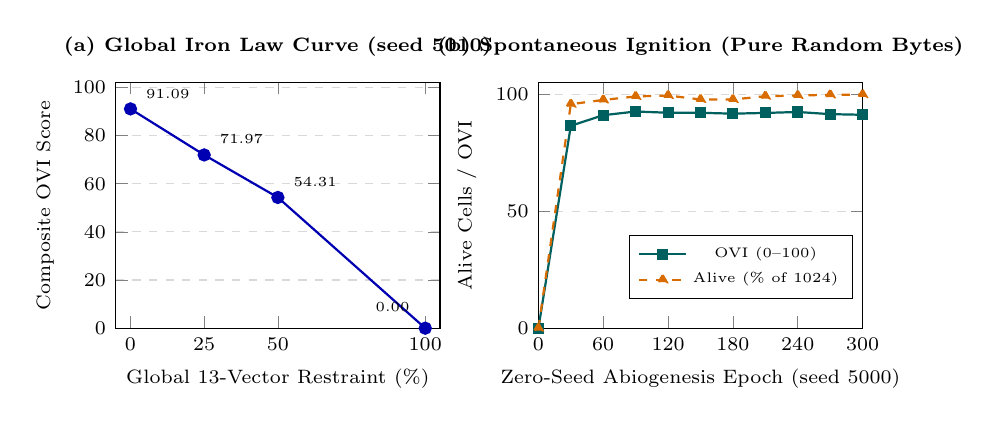
\begin{tikzpicture}
\begin{axis}[
  name=leftplot,
  width=0.47\textwidth,
  height=4.7cm,
  xlabel={Global 13-Vector Restraint (\%)},
  ylabel={Composite OVI Score},
  xmin=-5, xmax=105, ymin=0, ymax=102,
  xtick={0,25,50,100},
  ymajorgrids=true,
  grid style={dashed,gray!30},
  tick label style={font=\scriptsize},
  label style={font=\scriptsize},
  title style={font=\scriptsize\bfseries},
  title={(a) Global Iron Law Curve (seed 5010)}
]
\addplot[thick, blue!70!black, mark=*, mark size=2pt] coordinates {
  (0, 91.09)
  (25, 71.97)
  (50, 54.31)
  (100, 0.00)
};
\node[font=\tiny, anchor=south west] at (axis cs:2,91.5) {91.09};
\node[font=\tiny, anchor=south west] at (axis cs:27,72.5) {71.97};
\node[font=\tiny, anchor=south west] at (axis cs:52,54.8) {54.31};
\node[font=\tiny, anchor=south east] at (axis cs:98,3.0) {0.00};
\end{axis}

\begin{axis}[
  at={(leftplot.east)}, anchor=west, xshift=1.25cm,
  width=0.47\textwidth,
  height=4.7cm,
  xlabel={Zero-Seed Abiogenesis Epoch (seed 5000)},
  ylabel={Alive Cells / OVI},
  xmin=0, xmax=300, ymin=0, ymax=105,
  xtick={0,60,120,180,240,300},
  ymajorgrids=true,
  grid style={dashed,gray!30},
  tick label style={font=\scriptsize},
  label style={font=\scriptsize},
  title style={font=\scriptsize\bfseries},
  legend style={font=\tiny, at={(0.97,0.12)}, anchor=south east},
  title={(b) Spontaneous Ignition (Pure Random Bytes)}
]
\addplot[thick, teal!75!black, mark=square*, mark size=1.6pt] coordinates {
  (0,0.00) (30,86.56) (60,91.08) (90,92.66) (120,92.13)
  (150,92.11) (180,91.74) (210,92.05) (240,92.46) (270,91.53) (300,91.26)
};
\addlegendentry{OVI (0--100)}
\addplot[thick, orange!85!black, dashed, mark=triangle*, mark size=1.7pt] coordinates {
  (0,0.0) (30,95.8) (60,97.6) (90,99.1) (120,99.5)
  (150,97.8) (180,97.8) (210,99.2) (240,99.5) (270,99.8) (300,99.9)
};
\addlegendentry{Alive (\% of 1024)}
\end{axis}
\end{tikzpicture}
\caption{Measured empirical curves from AUTOPHAGE (\code{results/07_castration_ablation_13vec.csv} and \code{results/03_abiogenesis_zero_seed.txt}): (a)~strictly monotone Iron Law decline across global 13-vector restraint levels; (b)~spontaneous zero-seed abiogenesis ignition from $1{,}024$ pure random bytes.}
\label{fig:curves}
\end{figure}

Figure~\ref{fig:curves}(a) shows the monotone Iron Law curve across global restraint levels ($91.09 \to 71.97 \to 54.31 \to 0.00$, all $30$ ablation runs $\le 2.02 \times 10^{-16}$ drift); all $13/13$ individual restraints at $100\%$ score strictly below \code{GLOBAL_FERAL_0} ($91.09$), ranging from \code{SLOWING} ($0.00$) and \code{MINIMIZING} ($62.23$) to \code{SILOING} ($90.55$). Table~\ref{tab:stats} summarizes the preregistered confirmatory paired suite across all $N=24$ locked held-out seeds ($5000$--$5023$; $10{,}000$ sign-flip permutations with Holm--Bonferroni correction across $m=3$ hypotheses).

\begin{table}[t]
\centering
\caption{Confirmatory locked paired statistical suite ($N=24$, seeds $5000$--$5023$, $16\times 16$, $100$ epochs; \code{results/06_paired_stats_n24.txt}).}
\label{tab:stats}
\scriptsize
\renewcommand{\arraystretch}{1.15}
\begin{tabular}{@{}lrrrrrrr@{}}
\toprule
\textbf{Preregistered Hypothesis ($N=24$)} & \textbf{Mean A} & \textbf{Mean B} & \textbf{Mean Diff} & \textbf{Wins} & $\delta_{\text{pair}}$ & $p_{\text{signflip}}$ & $p_{\text{Holm}}$ \\
\midrule
H1. OVI: Feral vs.\ Castrated & $87.998$ & $22.686$ & $+65.312$ & $24/24$ & $+1.000$ & $0.00010$ & $0.00030$ \\
H2. Weismann Retro: Open vs.\ Lobotomized & $9920.042$ & $95.750$ & $+9824.292$ & $24/24$ & $+1.000$ & $0.00010$ & $0.00030$ \\
H3. Distinct Ribosomes: Feral vs.\ Delimited & $132.958$ & $2.625$ & $+130.333$ & $24/24$ & $+1.000$ & $0.00010$ & $0.00030$ \\
\bottomrule
\end{tabular}
\end{table}

\section{Unsolved Problems Mega-Atlas Non-Retirement Cross-Check}
\label{sec:atlas}

Cross-mapping AUTOPHAGE v1.5.0 against the $1{,}900$-problem \emph{Unsolved Problems Mega-Atlas} (\code{0thernes/unsolved-problems-mega-atlas}) confirms that \textbf{zero ($0 / 1{,}900$) overarching open problems are solved or retired}:
\begin{itemize}[leftmargin=1.5em,itemsep=2pt]
  \item \code{AI-045} (\emph{Open-Ended Artificial Life}, 1987): remains \textbf{OPEN}; AUTOPHAGE provides finite-grid OEE archive monotonicity (\code{Lean T41}) and $100$--$300$-epoch empirical measurements, not unbounded biological-scale novelty.
  \item \code{BIO-001} (\emph{Abiogenesis \& RNA-to-Ribosome Transition}, 1871): remains \textbf{OPEN}; computational self-replicator ignition inside an engineered x86-64 ISA is an analog, not prebiotic chemistry.
  \item \code{CHEM-052} (\emph{Non-Enzymatic RNA Replication Beyond Eigen's Error Threshold}, 1971): remains \textbf{OPEN}; algebraic $\mathbb{F}_{2^8}$ Cauchy MDS recovery (\code{Lean T15}--\code{T16}) is digital erasure coding, not RNA catalysis.
  \item \code{SYS-009} (\emph{Formal Cybernetic Theory of Multi-Scale Agency \& Autopoiesis}, 1948): remains \textbf{OPEN}; exact $5$-pool ledger conservation (\code{Lean T29a}, \code{T30}) and $2$-adic kin sensing (\code{Lean T25a}) do not constitute a general physical derivation of Markov blankets.
\end{itemize}

\section{Threats to Validity, Limitations, and Real-vs-Metaphor Boundary}
\label{sec:limits}

Full limitations are detailed in \code{LIMITATIONS.md}. Four principal threats to validity bound interpretation: (1)~\emph{Biological metaphor and calorimetry boundary:} terms such as ``ribosome'', ``Weismann barrier'', ``Planarian regeneration'', and ``digital cancer'' name exact C11/x86-64 algorithms and carry zero wet-lab biological identity; bit-erasure accounting counts logical bits overwritten in software, whereas physical CMOS execution dissipates far above $k_B T \ln 2$ per gate. (2)~\emph{Unformalized JIT encoding:} Lean~4.35.0 proves arithmetic mask and gas bounds (\code{Lean T26}--\code{T28}, \code{T48}) on \code{Spec.lean} models, while raw x86-64 instruction encoding relies on differential oracle testing (\code{Gate T04}, \code{Gate T09}), $10^6$-call canary fuzzing (\code{Gate T05}), libFuzzer (\code{test/fuzz_jit_libfuzzer.c}), and ASan/UBSan rather than a verified compiler backend. (3)~\emph{Finite scale \& single-thread determinism:} experiments run on $16\times 16$ or $32\times 32$ tori for $100$--$300$ epochs at \code{threads=1} to guarantee exact cross-OS SHA-256 identity. (4)~\emph{Single-hardware silicon profile and Windows \tcode{bwrap} boundary:} bare-metal GFNI timings were measured on one Intel Core Ultra~9 275HX, and Kernel \#6 (\code{lean4lean} + \code{bwrap} comparator) runs on Ubuntu Linux CI rather than native Windows.

\section{Reproducibility, Provenance, AI Disclosure, and Licensing}
\label{sec:repro}

\subsection{Reproducibility, Preservation, and Cryptographic Provenance}
From a clean clone of \url{https://github.com/0thernes/autophage} (interactive Lean~4 proof blueprint portal at \url{https://0thernes.github.io/autophage/}), running \code{pwsh -File build.ps1} (Windows) or \code{bash build_linux.sh} (Linux) builds all binaries, executes all $19/19$ falsification gates and $6/6$ planted mutants, and checks all $56$ Lean~4.35.0 theorems. Full multi-kernel replay runs via \code{scripts/verify_lean_multikernel.ps1} (Windows) or \code{lake check --paranoid \&\& lake comparator --config comparator.json --paranoid} (Ubuntu Linux) alongside \code{scripts/test_lean_negative.py} ($5/5$ live negative elaboration and axiom-tamper rejections). Independent property verification (\code{scripts/prop_check.py}), README axiom parity (\code{scripts/check_readme_axioms.py}), live Crossref/DataCite/HTTP bibliography verification (\code{scripts/check_citations.py}, $17/17$ targets verified in \code{results/citation-audit.json} with $0$ retractions and $0$ title/author/year mismatches), interactive blueprint checks (\code{scripts/check_blueprint.py}), and clean-room arXiv PDF compilation (\code{scripts/build_paper.py}) complete with zero external package installs.

Artifact integrity is anchored across four independent layers: (1)~cryptographic SHA-256 manifests (\code{CHECKSUMS.sha256} and \code{data/MANIFEST.sha256}); (2)~dual third-party timestamps minted over \code{CHECKSUMS.sha256} via DigiCert RFC~3161 (\code{CHECKSUMS.sha256.tsr}) and $3$-calendar Bitcoin OpenTimestamps (\code{CHECKSUMS.sha256.ots}), verified in CI by \code{scripts/stamp_timestamps.py --verify}; (3)~Sigstore Rekor / SLSA build provenance attestations (\code{actions/attest-build-provenance@v2}) in GitHub Actions; and (4)~permanent source archival at Software Heritage (\code{swh:1:snp:6ea23803655df1f9679deb98d44efbf53321a393}).

\subsection{Peer-Review Status, AI-Assistance Disclosure, CRediT, COI, and Licensing}
\textbf{Peer-Review Status:} This preprint and software repository are independent research works and have \textbf{not undergone external peer review}.
\textbf{CRediT Authorship:} Alexander Stephen Donahue (Independent Researcher, Spokane, WA, USA; ORCID \code{0009-0006-8168-9648}) is sole author responsible for Conceptualization, Methodology, Investigation, Supervision, Project Administration, Software Architecture, Formal Verification Policy, and Final Accountability. Frontier AI research and coding assistants (Gemini / Antigravity and Claude) assisted with C11 implementation, Lean~4.35.0 proof refactoring, adversarial test scaffolding, and AMS-LaTeX drafting under human direction and multi-kernel machine verification (\code{docs/AI_DISCLOSURE.md}).
\textbf{Conflicts of Interest:} The author declares no competing financial or institutional interests and no external funding.
\textbf{Dual Open License (REUSE/SPDX):} Source code, Lean~4.35.0 proofs, scripts, and CI workflows are licensed under \textbf{Apache-2.0} (\code{LICENSE}); this white paper, figures, documentation, and result tables are licensed under \textbf{CC-BY-4.0} (\code{LICENSE-DOCS}), with machine-readable SPDX coverage in \code{REUSE.toml}.

\FloatBarrier
\bibliographystyle{amsplain}
\bibliography{refs}

\end{document}
